\begin{center}
\textbf{
\MakeUppercase{Приложение А}\\
\\
Результат проверки системой Антиплагиат}
\end{center}
\addcontentsline{toc}{section}{Приложение А Фрагменты исходного кода}

\begin{center}
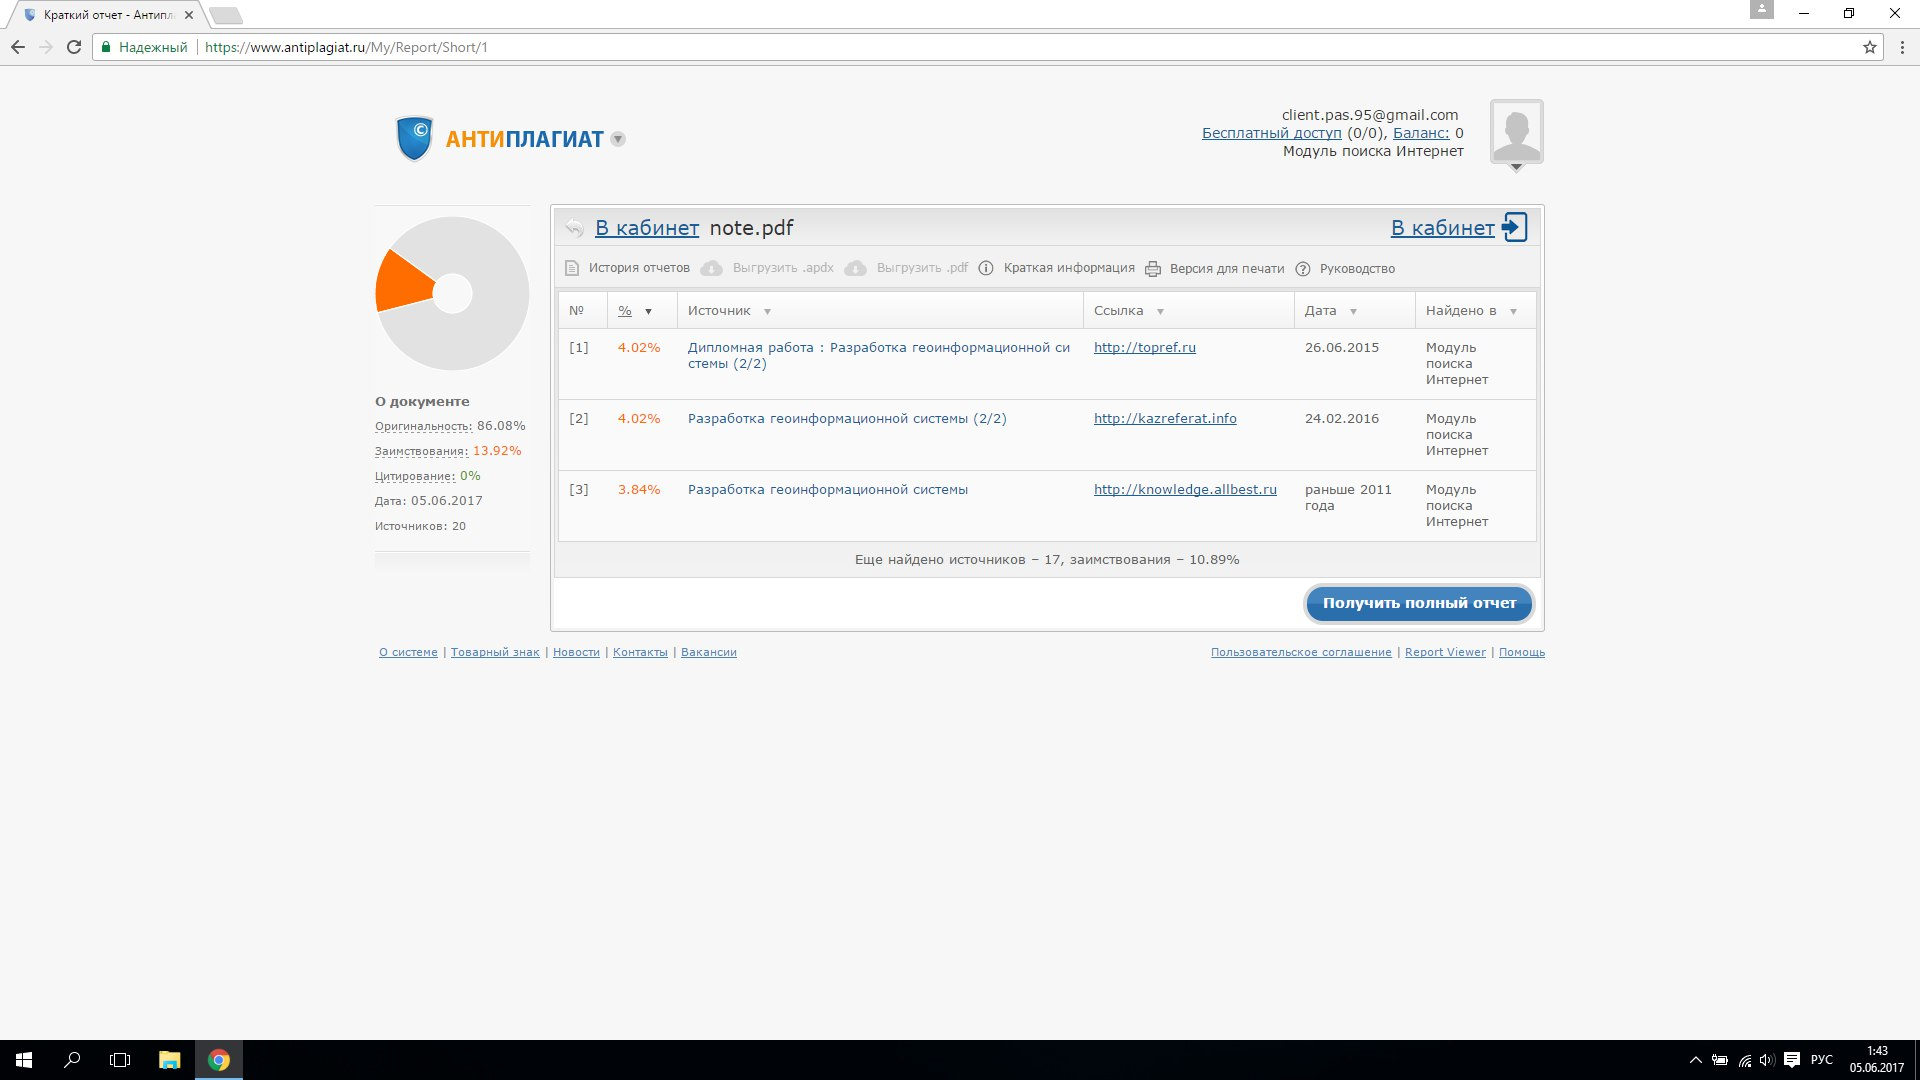
\includegraphics[scale=0.23]{antiplag.jpg}
\end{center}
\newpage

\begin{center}
\textbf{
\MakeUppercase{Приложение Б}\\
\\
Фрагменты исходного кода}
\end{center}
\addcontentsline{toc}{section}{Приложение А Фрагменты исходного кода}

\lstinputlisting[language=Python, caption={Модель для определения жанра композиции}]{appendices/model.py}

\lstinputlisting[language=Python, caption={Код для извлечение мел-частотных кепстральных коэффициентов}]{appendices/mfcc.py}

\lstinputlisting[language=Python, caption={Код для тренировки модели}]{appendices/train.py}

\lstinputlisting[language=Python, caption={Код для перемешивания большой выборки данных}]{appendices/mix_huge.py}
